\documentclass[a4paper]{article}

\usepackage{INTERSPEECH2021}
\usepackage[T1]{fontenc}
\usepackage{url}

\title{Regularising an LSTM Language Model on the Penn Treebank\\[3pt]
  \normalsize NLU course project -- language modelling (lab 4)}
\name{Andrea Giampietro (258237)}
\address{University of Trento}
\email{}

\begin{document}

\maketitle

\begin{abstract}
We study how far a one-layer LSTM language model can be pushed on the Penn Treebank by adding one regularisation
or optimisation technique at a time. Dropout and AdamW lower the test perplexity from 141.3 to 109.0; weight tying,
variational dropout and non-monotonically triggered averaged SGD (NT-AvSGD) bring a model trained with plain SGD
to 92.3.
\end{abstract}

\section{Introduction}

A language model estimates the probability of the next word given the previous ones, and its quality is measured
by the perplexity (PPL), the exponential of the average per-token cross-entropy on held-out text. This report
describes the language modelling project of the NLU course: a word-level LSTM \cite{hochreiter1997lstm} trained on
the Penn Treebank (PTB) \cite{marcus1993ptb,mikolov2010rnnlm} and improved incrementally, each step starting from the
best model of the previous one. Part~A adds dropout \cite{srivastava2014dropout} and replaces SGD with AdamW
\cite{loshchilov2019adamw}; part~B keeps SGD and adds the three techniques of AWD-LSTM \cite{merity2018awdlstm}:
weight tying, variational dropout and NT-AvSGD. The code is available at
\url{https://github.com/giampyhatesyou/Natural_Language_Processing}.

\section{Implementation details}

\textbf{Setup.} Every sentence is a sample ending with an \texttt{<eos>} token, the model predicts each next token
and the padding is masked out of the loss. All the models use 256-dimensional embeddings, one LSTM layer with 256
units and a linear output layer over the 10k-word vocabulary. Gradients are clipped to norm 5, training stops when
the dev PPL has not improved for 3 epochs, and the test set is always evaluated with the weights of the best dev
epoch.

\textbf{Part A.} The two dropout layers ($p=0.4$) act on the embeddings and on the LSTM outputs, before the output
layer; the AdamW experiment uses the same model.

\textbf{Weight tying} \cite{press2017tying,inan2017tying} reuses the embedding matrix $E$ as output layer,
$\mathrm{softmax}(E h_t + b)$: embedding and hidden sizes must match, and 2.56M of the 5.66M parameters disappear.

\textbf{Variational dropout} \cite{gal2016dropout} samples one Bernoulli mask per sequence and applies it at every
time step, on the same two positions as in part~A, instead of a new mask for every token.

\textbf{NT-AvSGD} follows Algorithm~1 of \cite{merity2018awdlstm} and wraps the SGD optimiser. Let
$v_1,\dots,v_t$ be the dev perplexities of the previous epochs and $v$ the current one; averaging starts the first
time that
\begin{equation}
  t > n \quad \text{and} \quad v > \min_{i \le t-n} v_i ,
\end{equation}
with non-monotone interval $n=5$: the model has to be worse than it was $n$ epochs before, so a single noisy epoch
is not enough. From then on, after the $m$-th SGD step the weights $w_m$ update a running mean of the iterates
\cite{polyak1992averaging},
\begin{equation}
  \bar w_m = \bar w_{m-1} + \tfrac{1}{m}\,(w_m - \bar w_{m-1}),
\end{equation}
and $\bar w$, not $w$, is validated, saved and tested. Early stopping is disabled before the trigger, which is
itself a plateau detector, and applied to $\bar w$ afterwards with a patience of 5 epochs.

\section{Results}

Tables~\ref{tab:partA} and~\ref{tab:partB} report the dev and test PPL of one run per configuration (seed 42,
trained on a T4 GPU), and Figure~\ref{fig:curves} the dev PPL after every epoch. In part~A, dropout lowers the test
PPL of the LSTM by 15.2 points and AdamW, on the same model, by a further 17.0, reaching 109.0. In part~B the tied
LSTM reaches 116.9 with 45\% fewer parameters (the untied LSTM of part~A, trained with a larger batch and learning
rate, reaches 141.3), and variational dropout gives the largest gain of the study ($-19.5$). NT-AvSGD lowers the
test PPL by a further 5.1 points, and the curves show where the gain comes from. Without early stopping before the
trigger, SGD keeps improving after epoch 58, where the run without NT-AvSGD stopped, and its best iterate reaches
97.6 dev PPL at epoch 72; averaging, triggered at epoch 74, brings the dev PPL to 94.9 and is still improving at
the 100-epoch limit. Of the 4.5 dev points gained over variational dropout, 1.8 come from the longer training and
2.7 from the averaging itself, in line with \cite{merity2018awdlstm}. The final model, trained with plain SGD, is
16.7 test points better than the AdamW model of part~A. As usually observed on PTB, the test PPL is lower than the
dev PPL for every model.

\begin{table}[t]
  \caption{Part A: perplexity on the dev and test sets. All models have 5.66M parameters and are trained with
  batch size 64; Ep.\ is the epoch of the selected checkpoint.}
  \label{tab:partA}
  \centering
  \setlength{\tabcolsep}{4.5pt}
  \begin{tabular}{l l c c c}
    \toprule
    Model & Optimiser & Ep. & Dev & Test \\
    \midrule
    LSTM            & SGD, lr 2           & 14 & 146.4 & 141.3 \\
    + dropout (0.4) & SGD, lr 2           & 67 & 131.1 & 126.0 \\
    + AdamW         & AdamW, lr $10^{-3}$ & 42 & 121.2 & \textbf{109.0} \\
    \bottomrule
  \end{tabular}
\end{table}

\begin{table}[t]
  \caption{Part B: perplexity on the dev and test sets. All models are trained with SGD (lr 1.5, batch size 32)
  and have 3.10M parameters; Ep.\ is the epoch of the selected checkpoint.}
  \label{tab:partB}
  \centering
  \begin{tabular}{l c c c}
    \toprule
    Model & Ep. & Dev & Test \\
    \midrule
    LSTM + weight tying         & 20  & 120.7 & 116.9 \\
    + variational dropout (0.4) & 55  & 99.4  & 97.4 \\
    + NT-AvSGD ($n=5$)          & 100 & 94.9  & \textbf{92.3} \\
    \bottomrule
  \end{tabular}
\end{table}

\begin{figure*}[t]
  \centering
  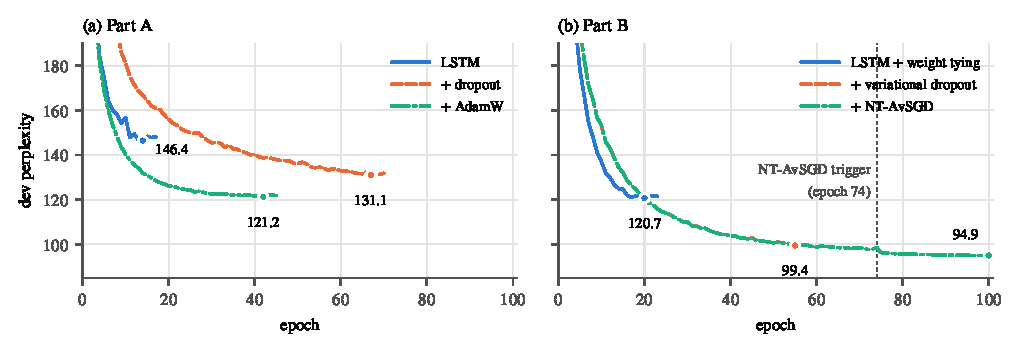
\includegraphics[width=\textwidth]{figures/lm_dev_ppl.pdf}
  \caption{Dev perplexity after every epoch (the first epochs, above 190, are cut). Dots mark the selected
  checkpoint of each run, i.e.\ its best dev epoch. The two runs with variational dropout coincide up to epoch 58,
  where early stopping ends the one without NT-AvSGD; with NT-AvSGD the averaged weights are evaluated from
  epoch 74 on.}
  \label{fig:curves}
\end{figure*}

\bibliographystyle{IEEEtran}
\bibliography{references}

\end{document}
